\section{Methodology}
\subsection{Statistical Concepts in Flood Frequency Hydrology}
Flood frequency hydrology involves fitting statistical distributions to annual flood peak data to model their probabilistic behavior. Frequency curves are then derived using Z-score transformations, which enables consistent interpretation of extreme event probabilities across different datasets. 

\subsubsection{Log-Pearson Type III (LP3) Distribution}
Among various statistical distributions, the Log-Pearson Type III (LP3) distribution is widely adopted for its ability to model the skewness inherent in annual flood peak data \citep{Singh_1998}. Let $Y$ represent independent and identically distributed (i.i.d) annual flood peak discharges:
$$Y = \{y_i \mid i = 1, 2, ..., n\}$$
 
Applying a logarithmic transformation:
$$x_i = \log_{10} (y_i)$$

The transformed data $x_i$ follows a Pearson Type III distribution, which is parametrized using its moments: the mean ($\mu$), standard deviation ($\sigma$) and skew ($\gamma$). The corresponding true parameters - location ($\xi$), shape ($\alpha$) and scale ($\beta$) - are computed as: 
\begin{align*}
    \xi = \mu - \frac{2 \sigma}{\gamma}, \quad \alpha = \frac{4}{\gamma^2}, \quad \beta = 0.5 \sigma \gamma 
\end{align*}

The probability density function (PDF) of the LP3 distribution is given by:
$$f_{\text{LP3}}(y_i \mid \mu, \sigma, \gamma) = f_{\text{gamma}} (x_i - \xi; \alpha, \beta) \cdot J$$
where $f_{\text{gamma}}$ denotes the gamma distribution, and $J$ is the Jacobian determinant:
$$J = \bigg| \frac{\partial (y_i)}{\partial x_i} \bigg|  = \bigg| \frac{\partial \log_{10} (y_i)}{\partial y_i} \bigg| = \frac{1}{y_i \cdot \ln(10)}$$

\subsubsection{Z-scores Transformation}
\label{sec:z_scores}
In hydrology, the Annual Exceedance Probability (AEP) is usually used to describe the likelihood of extreme events. It is defined as he probability that a particular hydrological event will be equaled or exceeded in any given year:
$$\text{AEP} = 1 -q$$
where $q$ is the cumulative probability associated with the quantile. For example, a quantile $q=0.99$ corresponds to an AEP of 1\%, meaning there’s a 1\% chance that the event magnitude will be exceeded.

Z-scores are used to standardize event probabilities. The Z-score represents the number of standard deviations by which a value lies from the mean in a standard normal distribution. For a given quantile $q$, the Z-score is calculated as:
$$Z(q) = -\Phi^{-1}(1-q) = -\Phi^{-1}(\text{AEP})$$
where $\Phi^{-1}$ is the Percent Point Function (PPF), or the inverse of the Cumulative Distribution Function (CDF) of the standard normal distribution.

\subsection{Maximum Likelihood Estimation (MLE)}
In the classical approach, the parameters of distributions ($\mu$, $\sigma$ and $\gamma$ for LP3) are estimated using the Maximum Likelihood Estimation (MLE) method. The likelihood function represents the probability of observing the data, $Y =(y_1, y_2,..., y_n)$, conditional on the distribution parameters: 
$$L (Y \mid \mu, \sigma, \gamma) =\prod_{i=1}^n f_{\text{LP3}} (y_i \mid \mu, \sigma, \gamma)$$

The natural logarithm of the likelihood simplifies the computation: 
$$\log L (Y \mid \mu, \sigma, \gamma) =\sum_{i=1}^n \big[\log f_{\text{gamma}} (x_i - \xi; \alpha, \beta) - \log \big(y_i \cdot \ln(10) \big) \big]$$

The parameters are estimated by minimizing the negative log-likelihood, a process that converts the maximization of the likelihood function into a minimization problem. The Nelder-Mead optimization method is employed for this purpose, ensuring efficient and robust estimation of the LP3 parameters.

\subsection{Bayesian Estimation Analysis}
In Bayesian analysis, parameter uncertainties are quantified through prior distributions  $\pi(\theta)$, where $\theta = \{\mu, \sigma, \gamma\}$ for LP3. Combining these priors with the likelihood function, $L (Y \mid \theta)$, derived from the observed data, the posterior distribution is:
$$ \pi (\theta \mid Y) = \frac{L (Y \mid \theta) \pi(\theta)}{\int L (Y \mid \theta) \pi(\theta) d\theta}$$
Since the integral in the denominator is generally intractable, Markov Chain Monte Carlo (MCMC) methods are used to approximate the posterior distribution through iterative sampling. To efficiently explore the parameter space and overcome potential convergence issues, we implement an adaptive Differential Evolution Markov Chain with Snooker updater (DE-MCzS) algorithm, as utilized in the BestFit software. The schematic diagram of the Bayesian framework is illustrated in Figure \ref{fig:DE-MCzS}. 

Unlike traditional MCMC methods that rely on a single chain, differential evolution markov chains maintain a population of chains that evolve collectively. This population-based approach allows chains to share information with candidate proposals informed by the states of other chains, thereby enhancing the algorithm's ability to navigate complex posterior landscapes. The DE-MCzS algorithm incorporates a snooker updater to further improve mixing and avoid local convergence traps \citep{Cheng_2014, Cheng_2014_b, Braak_2018}. The snooker updater generates proposals orthogonal to the chain's current trajectory. It leverages line projections to focus exploration on less-visited regions of the parameter space. The combination of differential evolution strategies and adaptive updates makes DE-MCzS effective and robust in Bayesian inference problems that are high-dimensional or involve multimodal distributions.

\begin{figure*}[ht!]
    \centering
    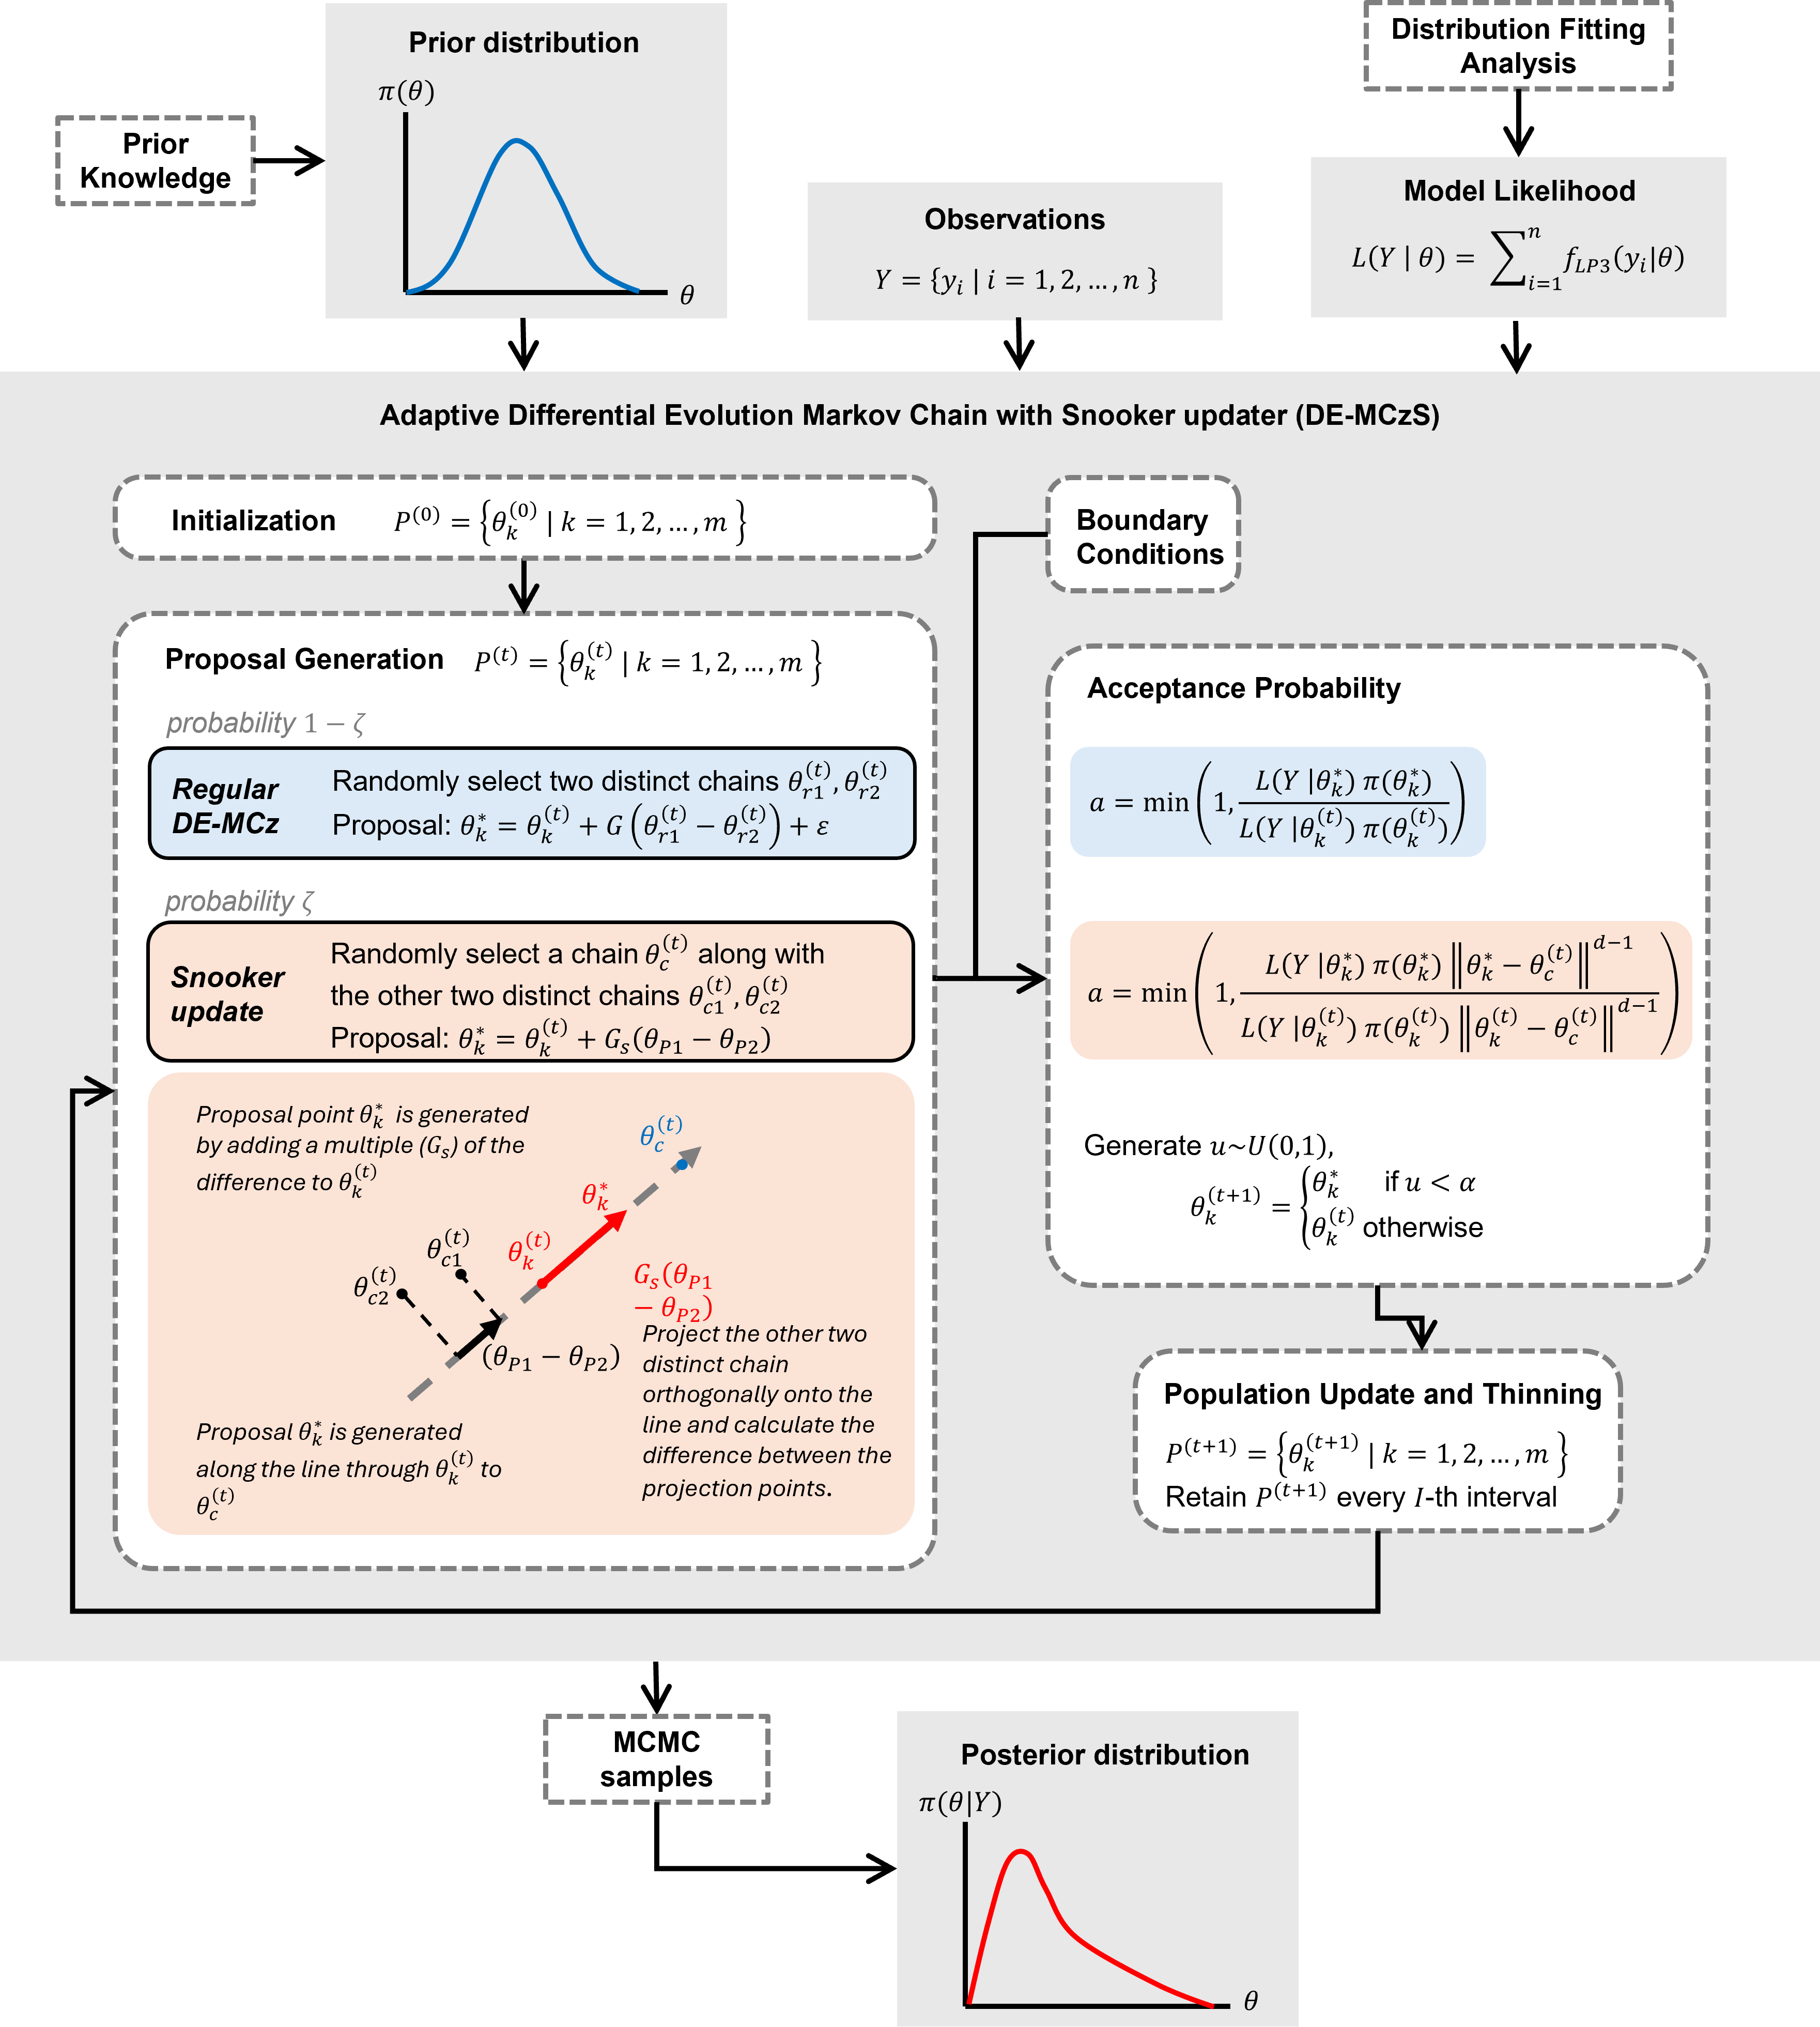
\includegraphics[width=1\linewidth]{_plots/DE-MCzS.png}
    \caption{Schematic representation of the Adaptive Differential Evolution Markov Chain with Snooker Update (DE-MCzS) algorithm. The diagram illustrates the Bayesian framework, including the prior distribution $\pi(\theta)$, the likelihood function $L(Y \mid \theta)$, and the posterior distribution $\pi(\theta \mid Y)$. Key steps of the algorithm are shown, such as initialization, proposal generation (regular and snooker updates), acceptance probability calculation, and posterior sampling.}
    \label{fig:DE-MCzS}
\end{figure*}

\subsubsection{Adaptive Differential Evolution Markov Chain with Snooker updater (DE-MCzS)}
\paragraph{Initialization}
The algorithm begins by initializing a population $P^{(0)}$ of $m$ chains, each containing a parameter vector $\theta_k^{(0)}$ sampled from the prior distribution:
$$P^{(0)} = \{{\theta_k}^{(0)}\mid k =1,2, ...,m\}$$

\paragraph{Proposal Generation} 
At iteration $t$, chain $k$ generates a proposal $\theta_k^*$, either through a regular DE-MCz update, or snooker update with a specified probability $\zeta$ (commonly set to $0.1$).

\paragraph{Regular DE-MCz Update}
The differential evolution strategy generates proposals by randomly selecting two distinct chains, $\theta_{r1}^{(t)}$ and $\theta_{r2}^{(t)}$ , and computing:
$$\theta_k^* = \theta_k^{(t)} + G\big( \theta_{r1}^{(t)} -\theta_{r2}^{(t)} \big) + \epsilon$$
where $G$ is a scaling factor and $\epsilon$ is a small perturbation term to maintain ergodicity and avoid premature convergence.

The scaling factor $G$ is determined based on a probability threshold $\delta$ and the jump parameter $\gamma$, as follows:
$$G = \begin{cases} 
1, & \text{with probability } \delta \\ 
\gamma, & \text{with probability } (1 - \delta) 
\end{cases}$$
where $\delta$ is typically set to $0.1$, and $\gamma$ is calculated as $\gamma = \frac{2.38}{\sqrt{2j}}$, with $j$ being the dimensionality of the parameter vector $\theta$. 

In BestFit, the perturbation $\epsilon$ is generated using a PPF-based noise term with power transformation:
$$\epsilon = (\Phi^{-1}(U))^p$$
where $\Phi^{-1}$ is the PPF (inverse CDF) of the standard normal distribution, $U \sim \text{Uniform} (0, 1)$, and $p$ is the exponent representing the number of parameters.
In this study, however, we adopt the Gaussian noise term for  $\epsilon$:
$$\epsilon \sim N(0, \sigma^2I)$$
where $I$ is the identity matrix, and $\sigma^2$ is the variance which is typically set to a small value such as $10^{-3}$.

\paragraph{Snooker Update}
In the snooker update, a chain $\theta_c^{(t)}$ is selected at random from the population. 
The proposal is generated along the line through $\theta_k^{(t)}$ to $\theta_{c}^{(t)}$, which is defined as:
$$\mathbf{l} = \theta_k^{(t)} - \theta_{c}^{(t)}$$
and its squared norm is:
$${\parallel\mathbf{l}\parallel}^2 = \mathbf{l}^\top \mathbf{l}$$
Two additional chains, $\theta_{c1}^{(t)}$ and $\theta_{c2}^{(t)}$, are selected, and their orthogonal projections onto the line $\mathbf{l}$ are calculated as:
$$\theta_{P1} = \theta_{c}^{(t)} + \frac{(\theta_{c1}^{(t)} - \theta_{c}^{(t)})^\top \mathbf{l}}{{\parallel\mathbf{l}\parallel}^2}\mathbf{l}, \quad \theta_{P2} = \theta_{c}^{(t)} + \frac{(\theta_{c2}^{(t)} - \theta_{c}^{(t)})^\top \mathbf{l}}{{\parallel\mathbf{l}\parallel}^2}\mathbf{l}$$
The proposal is then generated along the line $\mathbf{l}$ as:
$$\theta_k^* = \theta_k^{(t)} + G_s( \theta_{P1} - \theta_{P2})$$
where $G_s$ is a snooker-specific scaling factor sampled from a uniform distribution, typically $G_s \sim \text{Uniform}(1.2, 2.2)$.


\paragraph{Boundary Conditions}
Any proposed parameter vector $\theta_k^*$ that falls outside the feasible bounds defined by the prior distributions is automatically rejected to ensure the validity of the samples.

\paragraph{Acceptance Probability}
The acceptance of the proposed parameter vector $\theta_k^*$ is determined using the Metropolis-Hastings criterion. For the regular DE-MCz update, the acceptance probability $\alpha$ is calculated as:

$$a = \min \bigg(1, \frac{L(Y \mid \theta_k^*) \cdot \pi(\theta_k^*)}{L(Y \mid \theta_k^{(t)}) \cdot \pi(\theta_k^{(t)})}\bigg)$$

For the snooker update, the acceptance probability accounts for the change in volume due to the move being along a line, and is given by:
$$a = \min \bigg(1, \frac{L(Y \mid \theta_k^*) \cdot \pi(\theta_k^*) \cdot \parallel \theta_k^* - \theta_c^{(t)}\parallel ^{d-1}}{L(Y \mid \theta_k^{(t)}) \cdot \pi(\theta_k^{(t)}) \cdot \parallel \theta_k^{(t)} - \theta_c^{(t)}\parallel ^{d-1}}\bigg)$$
where $d$ is the dimensionality of the parameter space.

A uniform random number $u \sim \text{Uniform}(0, 1)$ is generated, and the chain is updated as:
$$\theta_k^{(t+1)} = 
\begin{cases} 
\theta_k^*, & \text{if } u < \alpha\\ 
\theta_k^{(t)}, & \text{otherwise} 
\end{cases}$$

\paragraph{Population Update and Thinning}
After all chains have been updated, the population becomes:
$$P^{(t+1)} = \{ \theta_k^{(t+1)}\mid k =1,2, ...,m\}$$
This updated population serves as the starting point for the next iteration. 

To reduce autocorrelation and improve statistical properties of MCMC samples, thinning is applied by retaining every $I$-th iteration:
$$\text{Retain sample at iteration } t \text{ if }t = zI, \quad z \in \mathbb{Z}^+$$
Additionally, an initial burn-in period is discarded to allow the chains to converge to the target distribution. At the conclusion of the simulation, a total of $N = 10,000$ samples are stored as the MCMC samples, which provides a comprehensive representation of the posterior distribution.

\subsubsection{Posterior Mode}
The posterior mode identifies the parameter values $\theta_{\text{mode}}$ that maximize the posterior probability density:
$$\theta_{\text{mode}} = \arg\max_{\theta} \pi(\theta \mid Y)$$

To simplify computations, the log-posterior is typically maximized instead:
$$\log \pi(\theta \mid Y) = \log L(Y \mid \theta) + \log \pi(\theta)$$

In cases where the prior distribution $\pi(\theta )$ is uniform or weakly informative, $\log \pi(\theta)$ becomes constant or negligible. As a result, the computation reduces to maximizing the log-likelihood:
$$\theta_{\text{mode}} = \arg\max_{\theta} \log L(Y\mid \theta)$$

Once $\theta_{\text{mode}}$ is computed, the posterior mode for a given quantile $q$ is calculated using the PPF:
$$\big\{F^{-1} (q_j \mid \theta_{\text{mode}}) \mid j = 1, 2, ..., M\big\}$$
where $F^{-1}$ is the PPF (inverse CDF) of the LP3 distribution, and $q_j$ represents the desired quantile value for $M$ quantiles of interest.

\subsubsection{Posterior Predictive and Credible Intervals}
The posterior predictive distribution evaluates the probability of future observations $\tilde{Y}$, conditioned on the observed data $Y$. This distribution accounts for both uncertainty in parameter estimates and variability in the data: 
$$\pi (\tilde{Y} \mid Y)= \int \pi(\tilde{Y} \mid \theta)\pi(\theta\mid Y) d\theta$$

Due to the intractability of this integral, the posterior predictive distribution is usually approximated through sampling. A logarithmic binning approach is adopted, as employed in BestFit, to efficiently capture a wide range of predictive values.

For each desired quantile $q_j$, PPF is computed for posterior samples $\theta^{(s)}$ obtained from MCMC samples: 
$$\big\{F^{-1} (q_j \mid \theta^{(s)}) \mid j = 1, 2, ..., M\big\}$$

The PPF values for all quantiles are transformed to the logarithmic scale. This range is divided into $B = 20$ bins using the minimum and maximum values:
$$\text{min PPF} = \log \big(\min \big\{F^{-1} (q_j \mid \theta^{(s)} ) \mid j = 1, 2, ...M \big\}\big)$$
$$\text{max PPF} = \log \big(\max \big\{F^{-1} (q_j \mid \theta^{(s)}) \mid j = 1, 2, ...M \big\}\big)$$

The bin edges represent future observations $\tilde{Y}$:
$$ \{\tilde{Y}\} = \big\{ \text{min PPF}, \text{min PPF}+ 10^{\frac{\text{max PPF} - \text{min PPF}}{B-1}}, ..., \text{max PPF} \big\}$$

For each bin $\tilde{Y}$, the CDF is used to compute the probability that $Y$ takes a value less than or equal to $\tilde{Y}$, given each sampled parameter set $\theta^{(s)}$. The averaged value across all samples is:
$$q({\tilde{Y}}) = \frac{1}{N} \sum_{s=1}^N F(\tilde{Y} \mid \theta^{(s)})$$
where $F$ is the CDF of the LP3 distribution. This quantile $q({\tilde{Y}})$ can be transformed into Z-scores $Z({\tilde{Y}})$ as describes in Section \ref{sec:z_scores}. 

Once Z-scores are computed for all bins, interpolation is used to estimate posterior predictive values for each desired quantile $q_j$:
$$\big \{\text{Interp} \big(Z(q_j)), \{Z({\tilde{Y}})\}, \{\tilde{Y}\}\big) \mid j = 1, 2, ..., M \big\}$$

For each quantile, credible intervals are numerically determined from the sampled PPF values. To construct a $(1 - 2a) \times 100\%$ credible interval, the bounds are defined as::
$$\text{Lower bound}: \text{Percentile} \big(a \cdot 100 \big)$$
$$\text{Upper bound}: \text{Percentile} \big((1-a) \cdot 100 \big)$$

\subsection{Non-stationarity}
\label{sec:nsffa}
In the Bayesian FFA described earlier, the observed data $Y = \{y_i \mid i = 1, 2, ..., n\}$ is assumed to be independent and identically distributed
(i.i.d). However, this assumption may not hold true in a non-stationary environment, particularly under the influence of climate change. Non-stationary flood frequency analysis (NSFFA) accounts for temporal variations in the parameter vectors $\theta$, resulting in a time-dependent likelihood function \citep{Smith_2024}:
$$L (Y \mid \theta) =\prod_{t=1}^T f_{\text{LP3}} (y_i \mid \theta_t)$$
where $\theta_t$ is the parameter set for time step $t$, which allows the distribution to evolve over time.

In this study, non-stationarity is considered only with respect to the location parameter $\mu$, as temporal variations in the scale parameter $\sigma$  and shape parameter $\gamma$ require substantial long-term data, which is often difficult to obtain \citep{Cheng_2014_b}. Temporal changes in $\mu$ are modeled using linear and exponential trends:
\begin{align*}
    \text{linear: } & \mu_t = \beta_0 + \beta_1 \cdot t\\
    \text{exponential: } & \mu_t = \beta_0 \cdot \exp (\beta_1 \cdot t)
\end{align*}
where $t$ is the time in years (with $t=0$ representing the first observed data point), $\beta_0$ is the intercept representing the initial location parameter at $t=0$, and $\beta_1$ is the coefficient controlling the strength of the trend over time. 

In NSFFA, each time step has a unique parameter set, which means there is a unique set of distribution properties over time. As a result, the exceedance probabilities of flow values also varies with time. A time index property is introduced in BestFit to determine the time step for evaluating the non-stationary frequency distribution \citep{Smith_2024}. 

\FloatBarrier
